\chapter{背景}
\label{background}

本章では本研究の背景について述べる.

\section{ネットワーク音楽演奏}
\label{background:nmp}
一概にネットワーク音楽演奏と呼んでも様々なものがある.
ここでは本研究で扱うネットワーク音楽演奏システムのスコープを定義づける.



ネットワーク音楽演奏で演奏を届ける手法は,VoIPアプリケーションのように音声の波形情報を処理し低遅延で届ける方法\cite{syncroom}\cite{lola}\cite{jacktrip},演奏情報をMIDIを使い楽器,音程,強度などに抽象化し,受信した機器が演奏データを元に音を合成するという方法\cite{rtpmidi}\cite{sourcenode}と,2種類の手法に分けることができる.

本研究では次の仕様のネットワーク音楽演奏システムを扱う.

\begin{itemize}
  \item 1対1の合計2人の演奏者を扱う.
  \item 演奏情報をMIDI形式で送受信する.
  \item 楽譜などの事前に演奏に関する情報はない.
  \item 最大160msの遅延が発生する.
\end{itemize}

\section{インテリジェントネットワーク音楽演奏}
ネットワーク音楽演奏システムの中でも単に現実の音楽演奏とできるだけ近づくようにAからBへと演奏情報を低遅延で正確に届けるだけでなく,遅延の対処するため,演奏の没入感を高めるためなど,ネットワーク音楽演奏の課題点を独自の手法で解決するシステムは多数存在する.
これらを\cite{impedence}では「Intelligent Networked Music Performance (インテリジェントネットワーク音楽演奏)」と呼んでいる.
\cite{tablanet}\cite{alexandraki:2014}\cite{alexandraki:2013} \cite{admet}

\section{Adaptive Metronome}
BattelloらによるAdaptive Metronome\cite{admet}\cite{admet:experiment}は,演奏者の演奏をリアルタイムで分析し,演奏者の演奏に合わせてメトロノームのテンポを変化させるシステムである.

\begin{figure}[htbp]
  \centering
  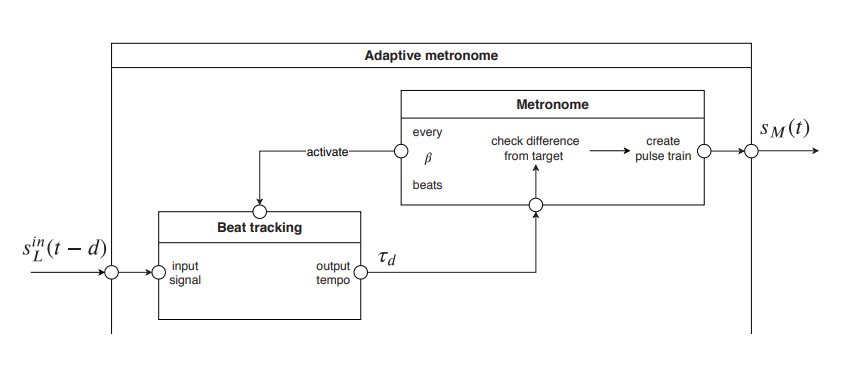
\includegraphics[width=0.8\linewidth]{src/admet.png}
  \caption{Adaptive Metronomeの実験\cite{admet}}
  \label{fig:admet}
\end{figure}

Adaptive Metronomeは親子構造を持っている.
親の演奏者は演奏すると同時にシステムはリアルタイムでその演奏の拍を推定し,子演奏者に音声と拍情報を送信する.
子演奏者のシステムはその情報を受取り,親演奏者の演奏に合わせてメトロノームのテンポを変化させる.
またこのときメトロノームの音は親から子への遅延を考慮して位相をずれして再生される.

こうすることで小演奏者に聞こえるメトロノームは親演奏者の遅延された演奏に関わらず,常に親演奏者の無遅延の演奏に合わせたテンポで再生される.
このシステムを用いた実験では120msの遅延下での演奏を行ったうえでも,被験者は抵抗を感じることなく演奏することができたという結果が得られた.\cite{admet}

\subsection{相互メトロノームの実験}
当初のAdaptive Metronomeの実験では,親演奏者の演奏を子演奏者が聴き,それに合わせて演奏するという形で実験が行われた.
後にBatteloらは親子構造を持たず,相互的にAdaptive Metronomeを聞きあう実験を行った.
実験の結果は現状まだ不十分であるが,このような相互的なシステムでもある程度の効果が得られることが示された.

% 以降は最後にメンション
\section{Tablanet}
Tablanet\cite{tablanet}は,タブラ奏者の演奏をリアルタイムで分析し,演奏者の演奏に合わせてタブラのテンポを変化させるシステムである.
\section{Alexandraki}
Alexandrakiらによる研究\cite{alexandraki:2013}\cite{alexandraki:2014}では,演奏者の演奏をリアルタイムで分析し,事前収録した演奏を実際の演奏に合わせて再生するシステムを提案している.
